%Here a lot is missing but for first start I have copied the graphics which content should be included here REFERENCE_numerical. Page 271 main reference \cite{numeric_method_book}
\subsection{Posing the problem} \label{sec: posingProblem}
To simplify our approach we look at a two-dimensional incompressible fluid. In this section we want to pose the problem by introducing the underlying mathematical equations and discuss the boundary conditions.

\subsubsection*{Underlying equations}
In our approach we simplify the problem to a two-dimensional incompressible viscous fluid in a rectangular domain box flowing from one side of the box to the other, encountering an obstacle in its path. The motion of the fluid is described by the \textit{incompressible Navier-Stokes equation}

\begin{align}
  \rho \left( \frac{\partial \textbf{u}}{\partial t}  + \textbf{u} \cdot \nabla \textbf{u} \right)- \mu \Delta \textbf{u}+ \nabla p =0 \label{eq: incompressNS} \\
  \nabla\cdot \textbf{u} = 0 \notag
\end{align}

where $\rho$ is the mass density (assumed constant), $\textbf{u} = (u,v)$ is the fluid velocity with horizontal component $u$ and vertical component $v$, $\mu$ is the dynamic viscosity of the fluid and $p$ is the pressure. The first equation encapsulates the momentum balance within the fluid, incorporating the effects of convection (velocity interaction and movement), diffusion (velocity spreading due to viscosity), and the pressure gradient's influence on the fluid motion, whereas the second equation, often termed the continuity equation, asserts the incompressibility of the fluid by ensuring the volume conservation within the flow. The equations can be adimensionalized to obtain the dimensionless \textit{Reynolds number} by looking at

\begin{align}
  \Tilde{\textbf{u}} = \frac{\textbf{u}}{U}, \quad \Tilde{p} = \frac{p}{\rho U^2}, \quad \Tilde{\textbf{x}} = \frac{\textbf{x}}{L}, \quad \Tilde{t} = \frac{U}{L}t
\end{align}

where the characteristic velocity $U$ and length $L$ are used. These quantities represent the typical velocity of the fluid and typical lengthscale. In practice they are taken to be the inflow velocity and the diameter of the object, respectively. Applying these change of variables to \cref{eq: incompressNS}, we get (dropping the tilde for readability):

\begin{align}
  \frac{\partial \textbf{u}}{\partial t} + \textbf{u} \cdot \nabla \textbf{u} - \frac{1}{\text{Re}} \Delta \textbf{u} + \nabla p = 0 \\
  \nabla\cdot\vf{u} = 0 \notag
\end{align}

where the Reynolds number $\Rey = \frac{\rho U L}{\mu}$ measures the ratio between the inertia of the flow and the viscosity of it.

\subsubsection*{Boundary conditions}
%The body is first time mentionend here but will be explained later
The domain $\Omega$ is the rectangular box without the obstacle. We call the horizontal direction $x$ and the vertical direction $y$-direction. In our study on the left side a laminar flow is coming into the domain. At the beginning the fluid inside the box is at rest. At the horizontal walls a slip condition is imposed and a free flow on the right side is assumed. Therefore we obtain as boundary conditions for the walls:

\begin{itemize}
  \item At time $t=0$, the fluid is at rest, and both velocity and pressure are zero.
  \item On the left side, the flow is incoming with a velocity equal to $U \mathbf{e}_x$, and the pressure satisfies the conditions $\frac{\partial p}{\partial x} = 0$.
  \item On the right side of the domain, the flow is free so that $\frac{\partial u}{\partial x} = \frac{\partial v}{\partial x} = 0$ and $p = 0$.
  \item On the horizontal sides, the walls are impenetrable, so that $v = 0$. A slip condition is imposed so that $\frac{\partial u}{\partial y} = 0$ and $\frac{\partial p}{\partial y} = 0$.
\end{itemize}

In order to accurately implement these boundary conditions, we made use of the \textit{ghost cell} method. This technique involves the addition of a layer of cells outside the domain (see \cref{fig: ghostCells}). These cells are used to approximate at first order the values of the velocity and pressure at the boundary for both Dirichlet and Neumann conditions

\begin{figure}[h]
  \centering
  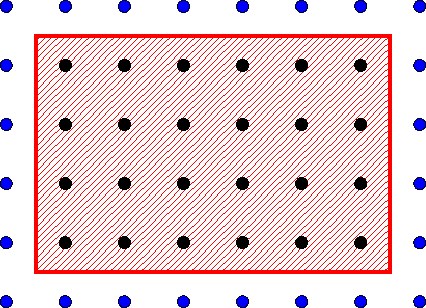
\includegraphics[width=0.5\textwidth]{0_graphics/methods/grid.pdf}
  \caption{The ghost cell method. The domain $\Omega$ is represented in red and the dots represent the grid cells, the black ones being the inner points and the blue ones, the ghost cells.}
  \label{fig: ghostCells}
\end{figure}

As an example, if $u_{0,j}$ denotes the horizontal component of $\vf{u}$ at the left boundary and height $j$ (counting from 0), then it will be approximated by $2U-u_{1,j}$, where $u_{1,j}$ is the horizontal component of $\vf{u}$ at the first cell inside the domain and the same height $j$. Similarly, we obtain values for $v_{0,j}$ and $p_{0,j}$ as

$$
  v_{0,j} = -v_{1,j}, \quad p_{0,j} = p_{1,j}
$$

The other boundaries are treated in the same way. It should be noted than when computing discrete derivatives, which involve the use of neighboring cells, the computations are carried out only with inner cells, which in turn use ghost cells. But the derivatives itself at ghost cells are never computed.

We discuss now the treatment of the boundary conditions on the object. In general dealing with the object is not an easy task. For simplicity, we model the presence of a solid body within a fluid by enforcing the fluid velocity to be zero at the boundaries that correspond to the shape of the body, which correspond to imposing a no-slip condition.
It is very worth-mentioning that the way we integrate the body has an influence on the flow. Especially to study the impacts of coatings or surface structure, our method, is not capable of including these effects, but in our approach we only want to observe the effect, and therefore prioritize simplicity for understanding over complexity for small details in the effect. If the reader is interested in delving deeper into the fluid-structure interactions, including the effects of surface modifications, we recommend consulting works in the field, such as those by Peskin \cite{Peskin1977ImmersedBM} or Schlichting and Gersten \cite{Schlichting2000BoundaryLayerT}.

\subsection{Difference Scheme} \label{sec: diffScheme}
In this section we discuss our numerical solver to integrate \cref{eq: incompressNS} together with the boundary conditions presented in above section. To simplify the equations, we use \textit{Chorin's projection method}. It was originally introduced by Alexandre Chorin in 1967 \cite{Chorin1967NumericalNS} as an efficient means of solving the incompressible Navier-Stokes equations.

The idea of the method is to first predict the velocities for the next time step by solving the advection and the diffusion term. With the intermediate velocity field we solve the Poisson equation with a finite difference method (described below). Finally, the \textit{projection step} is preformed, and the velocity field is updated with the new pressure field.
To ensure that the boundary conditions are met, we impose the conditions for the velocity right before solving the Poisson equation and at the end of each iteration. The boundary conditions for the pressure are imposed after solving the Poisson equation and before correcting the velocities in the projection step.

Next, we provide a summary of the steps in our method:
\begin{enumerate}
  \item $\displaystyle  \frac{\vf{u}^a-\vf{u}^n}{\Delta t} + \vf{u}^n \cdot \nabla \vf{u}^n = 0$
  \item $\displaystyle  \frac{\vf{u}^* - \vf{u}^a}{\Delta t} = \frac{1}{\Rey} \laplacian \vf{u}^n$
  \item Set the boundary conditions for the intermediate velocity field $\vf{u}^*$ and impose set the velocity field $\vf{u}^*$ inside the object to be zero (forcing term).
  \item $\displaystyle \laplacian p^{n} = \frac{1}{\Delta t}\nabla \cdot \vf{u}^*$
  \item Set the boundary conditions for the pressure $p^{n}$.
  \item $\displaystyle \vf{u}^{n+1} = \vf{u}^* - \Delta t\nabla p^{n}$
  \item Set the boundary conditions for the velocity field $\vf{u}^{n+1}$.
\end{enumerate}
From these equations, one can easily check that we have:
\begin{align*}
  \frac{\vf{u}^{n+1}-\vf{u}^n}{\Delta t} + \vf{u}^n \cdot \nabla \vf{u}^n - \frac{1}{\Rey} \laplacian \vf{u}^n + \nabla p^{n} & = 0 \\
  \nabla \cdot \vf{u}^{n+1}                                                                                                   & = 0
\end{align*}

In the following sections we will deepen in how do we compute each of the above steps in our method.

\subsubsection*{Semi-Lagrangian method}
% What is a Semi-Langrangian method
The Semi-Lagrangian method represents a powerful approach to solving fluid dynamics problems, particularly in the context of advection. Unlike Eulerian methods, which compute changes at fixed points in space, the Semi-Lagrangian (SL) method tracks the motion of fluid parcels. SL methods slightly differ from Lagrangian methods, as the word suggest. The second ones are rarely used in numerical methods because the particle trajectories become chaotic and wildly mixed in a short period of time. However, SL algorithms avoid this problem by `reinitializing' the Lagrangian coordinate system after each time step \cite{Boyd2001ChebyshevFourier}. There are several ways to implement a SL method, and we will describe the one we used in our method. Our goal in this subsection is on solving:

\begin{equation*}
  \frac{\mathrm{D}\vf{u}}{\mathrm{D}t} = \pdv{\vf{u}}{t} + \vf{u} \cdot \nabla \vf{u} = 0
\end{equation*}

The idea is to somehow discretize the material derivative. To do that, if we call $\vf{u}^n$ the current velocity field and $\vf{u}^a$ the velocity field after the convection step, we can write a difference formula as:

\begin{equation*}
  \frac{\vf{u}^a- \vf{u}^n}{\Delta t} + \vf{u}^n \cdot \nabla \vf{u}^n = 0
\end{equation*}

The following discretization for the material derivative is used:

\begin{equation*}
  \frac{\vf{u}(\vf{x}_{i,j},t^{n+1})  - \vf{u}(\vf{x}_{i,j} - \vf{u}(\vf{x}_{i,j},t^n)\Delta t,t^n)}{\Delta t}
\end{equation*}

The reader may rapidly notice that the point $\vf{x}_{i,j} - \vf{u}(\vf{x}_{i,j},t^n)\Delta$ will not in general be in the grid, and thus, we will not have the respective value of the velocity field. To solve this problem, we will make use of bilinear interpolation between the four (in 2D) nearest grid points to the point $\vf{x}_{i,j} - \vf{u}(\vf{x}_{i,j},t^n)\Delta t$. This will give us an approximation of the velocity field at the point $\vf{x}_{i,j} - \vf{u}(\vf{x}_{i,j},t^n)\Delta t$, which in turn will give us the convected velocity field $\vf{u}^a$.

Furthermore, to improve the accuracy of the method we use the back-and-forth method \cite{backforth}. This method first advects the velocity field using the method described above, and then advects back with opposite velocity $\vf{u}\to -\vf{u}$. With this we can have an estimate of the error we are comitting when comparing the last result with the initial position. Using this information we can correct the velocity field and obtain a more accurate result. The steps are reproduced below. In order to make things more clear, we will consider the general case:

\begin{equation*}
  \frac{\mathrm{D}\vf{\psi}}{\mathrm{D}t} = \pdv{\vf{\psi}}{t} + \vf{u} \cdot \nabla \vf{\psi} = 0
\end{equation*}

\begin{enumerate}
  \item Advect the field $\vf\psi^n$ with velocity $\vf{u}$ to obtain $\tilde{\vf{\psi}}^a$.
  \item Advect the field $\vf{\tilde{\psi}}^a$ with velocity $-\vf{u}$ to obtain $\vf{\bar{\psi}}^a$.
  \item Advect the field $\vf{\psi}^n + \frac{1}{2} (\vf{{\psi}}^n - \vf{\bar{\psi}}^a)$ with velocity $\vf{u}$ to obtain $\vf{\psi}^a$.
\end{enumerate}

\subsubsection*{Diffusion term}
As a second step we add diffusion using a 2nd order central differences. The diffusion term is given by:

\begin{equation*}
  \frac{\vf{u}^* - \vf{u}^a}{\Delta t} = \frac{1}{\Rey} \laplacian \vf{u}^n
\end{equation*}

Once discretized we get, for each $i$, $j$ in the grid:

\begin{equation*}
  \vf{u}^*_{i,j} = \vf{u}^a_{i,j} + \frac{\Delta t}{\Rey}\left( \frac{\vf{u}^n_{i+1,j} - 2\vf{u}^n_{i,j} + \vf{u}^n_{i-1,j}}{{(\Delta x)}^2} + \frac{\vf{u}^n_{i,j+1} - 2\vf{u}^n_{i,j} + \vf{u}^n_{i,j-1}}{{(\Delta y)}^2}\right)
\end{equation*}

As before, we write concisely the discretization in vector form but in practice we do it for each component of the velocity field separately.

\subsubsection*{Solving for the Poisson equation}\label{sec: solvingPoisson}
There are several efficient ways to compute the solution of the general Poisson equation $\Delta p = f$. In our case, we have to equip this equation with the boundary conditions $\partial_{\vf{n}}p=0$ on the left, top and bottom boundaries, and $p=0$ on the right boundary. We will use a finite difference method to solve this equation. The idea is to discretize the domain into a grid and use the finite difference method to solve the equation. We will use a 5-point stencil to approximate the Laplacian operator. The 5-point stencil is given by:

\begin{equation*}
  \laplacian p_{i,j} = \frac{p_{i+1,j} - 2 p_{i,j} + p_{i-1,j}}{{(\Delta x)}^2} + \frac{p_{i,j+1} - 2 p_{i,j} + p_{i,j-1}}{{(\Delta y)}^2}
\end{equation*}

If we set $\vf{p}:=(p_{11}, p_{12}, \ldots, p_{1n_y}, p_{21}, \ldots, p_{22}, \ldots, p_{2n_y},\ldots p_{n_xn_y})$, we can write our problem in matrix form as $\vf{A}\vf{p}=\vf{f}$, where $\vf{f}$ contains the discrete values of the right-hand side of the Poisson equation in the same order as $\vf{p}$, and $\vf{A}$ is a matrix that contains the coefficients of the Laplacian operator. Let's describe how we can build the matrix $\vf{A}$. Let $\vf{A}=\vf{X} + \vf{Y}$, where $\vf{X}$ and $\vf{Y}$ are the matrices that contain the coefficients of the Laplacian operator in the $x$ and $y$ directions, respectively. We can write $\vf{X}$ and $\vf{Y}$ as:

\begin{equation*}
  \vf{X} = \begin{pmatrix}
    -\vf{I}_{n_y} & \vf{I}_{n_y}   & \vf{0}         & \cdots       & \cdots         & \vf{0}         \\
    \vf{I}_{n_y}  & -2\vf{I}_{n_y} & \vf{I}_{n_y}   & \ddots       &                & \vdots         \\
    \vf{0}        & \vf{I}_{n_y}   & -2\vf{I}_{n_y} & \vf{I}_{n_y} & \ddots         & \vdots         \\
    \vdots        & \ddots         & \ddots         & \ddots       & \ddots         & \vf{0}         \\
    \vdots        &                & \ddots         & \vf{I}_{n_y} & -2\vf{I}_{n_y} & -\vf{I}_{n_y}  \\
    \vf{0}        & \cdots         & \cdots         & \vf{0}       & \vf{I}_{n_y}   & -3\vf{I}_{n_y} \\
  \end{pmatrix}\quad
  \vf{Y} = \begin{pmatrix}
    \vf{B} & \vf{0} & \cdots & \vf{0} \\
    \vf{0} & \vf{B} & \ddots & \vdots \\
    \vdots & \ddots & \ddots & \vf{0} \\
    \vf{0} & \cdots & \vf{0} & \vf{B} \\
  \end{pmatrix}
\end{equation*}

with

$$
  \vf{B} = \begin{pmatrix}
    -1     & 1      & 0      & \cdots & 0      \\
    1      & -2     & 1      & \ddots & \vdots \\
    0      & \ddots & \ddots & \ddots & 0      \\
    \vdots & \ddots & 1      & -2     & 1      \\
    0      & \cdots & 0      & 1      & -1     \\
  \end{pmatrix}\in\mathcal{M}_{n_y}(\mathbb{R})
$$

Both $\vf{X}$ and $\vf{Y}$ are block matrices, composed of $n_x$ matrices of size $n_y\times n_y$ each, which results in a matrix of size $n_xn_y\times n_xn_y$.
The boundary conditions (using ghost cells) on the pressure are applied at both the first and last block row of $\vf{X}$ and the first and last row of $\vf{Y}$.

In order to solve the resulting system, we have used the Cholesky decomposition, which requires the matrix to be symmetric and positive definite. The matrix $\vf{A}$ is symmetric, but it is not positive definite. In fact, it can be seen that it is negative definite. Thus, in our case, we will be solving the equivalent system $-\vf{A} \vf{p} = -\vf{f}$.


\subsubsection*{Updating velocities}

As a final step, we compute the gradient of the pressure field and update the velocity field. The gradient of the pressure field is computed using a 2nd order central differences. The update of the velocity field is given by:

\begin{equation*}
  \vf{u}_{i,j}^{n+1} = \vf{u}_{i,j}^* - \Delta t \left(
  \frac{p_{i+1,j}^{n} - p_{i,j}^{n}}{\Delta x}, \frac{p_{i,j+1}^{n} - p_{i,j}^{n}}{\Delta y}
  \right)
\end{equation*}

